\chapter{Conclusion and Future Directions}
\label{chap:conclusion}
% Discussion: remaining challenges, the benefits in another fields than oncology

new pipelines for new technology

gene annotation unification MANE

pan-cancer PTM
- reprocess the data
- kinase substrate library



With the map of \fref{fig:gbm-graphical-abstract}

longitudal study

overview of the next gbm confirmatory cohort

\begin{figure}[tb]
    \centering
    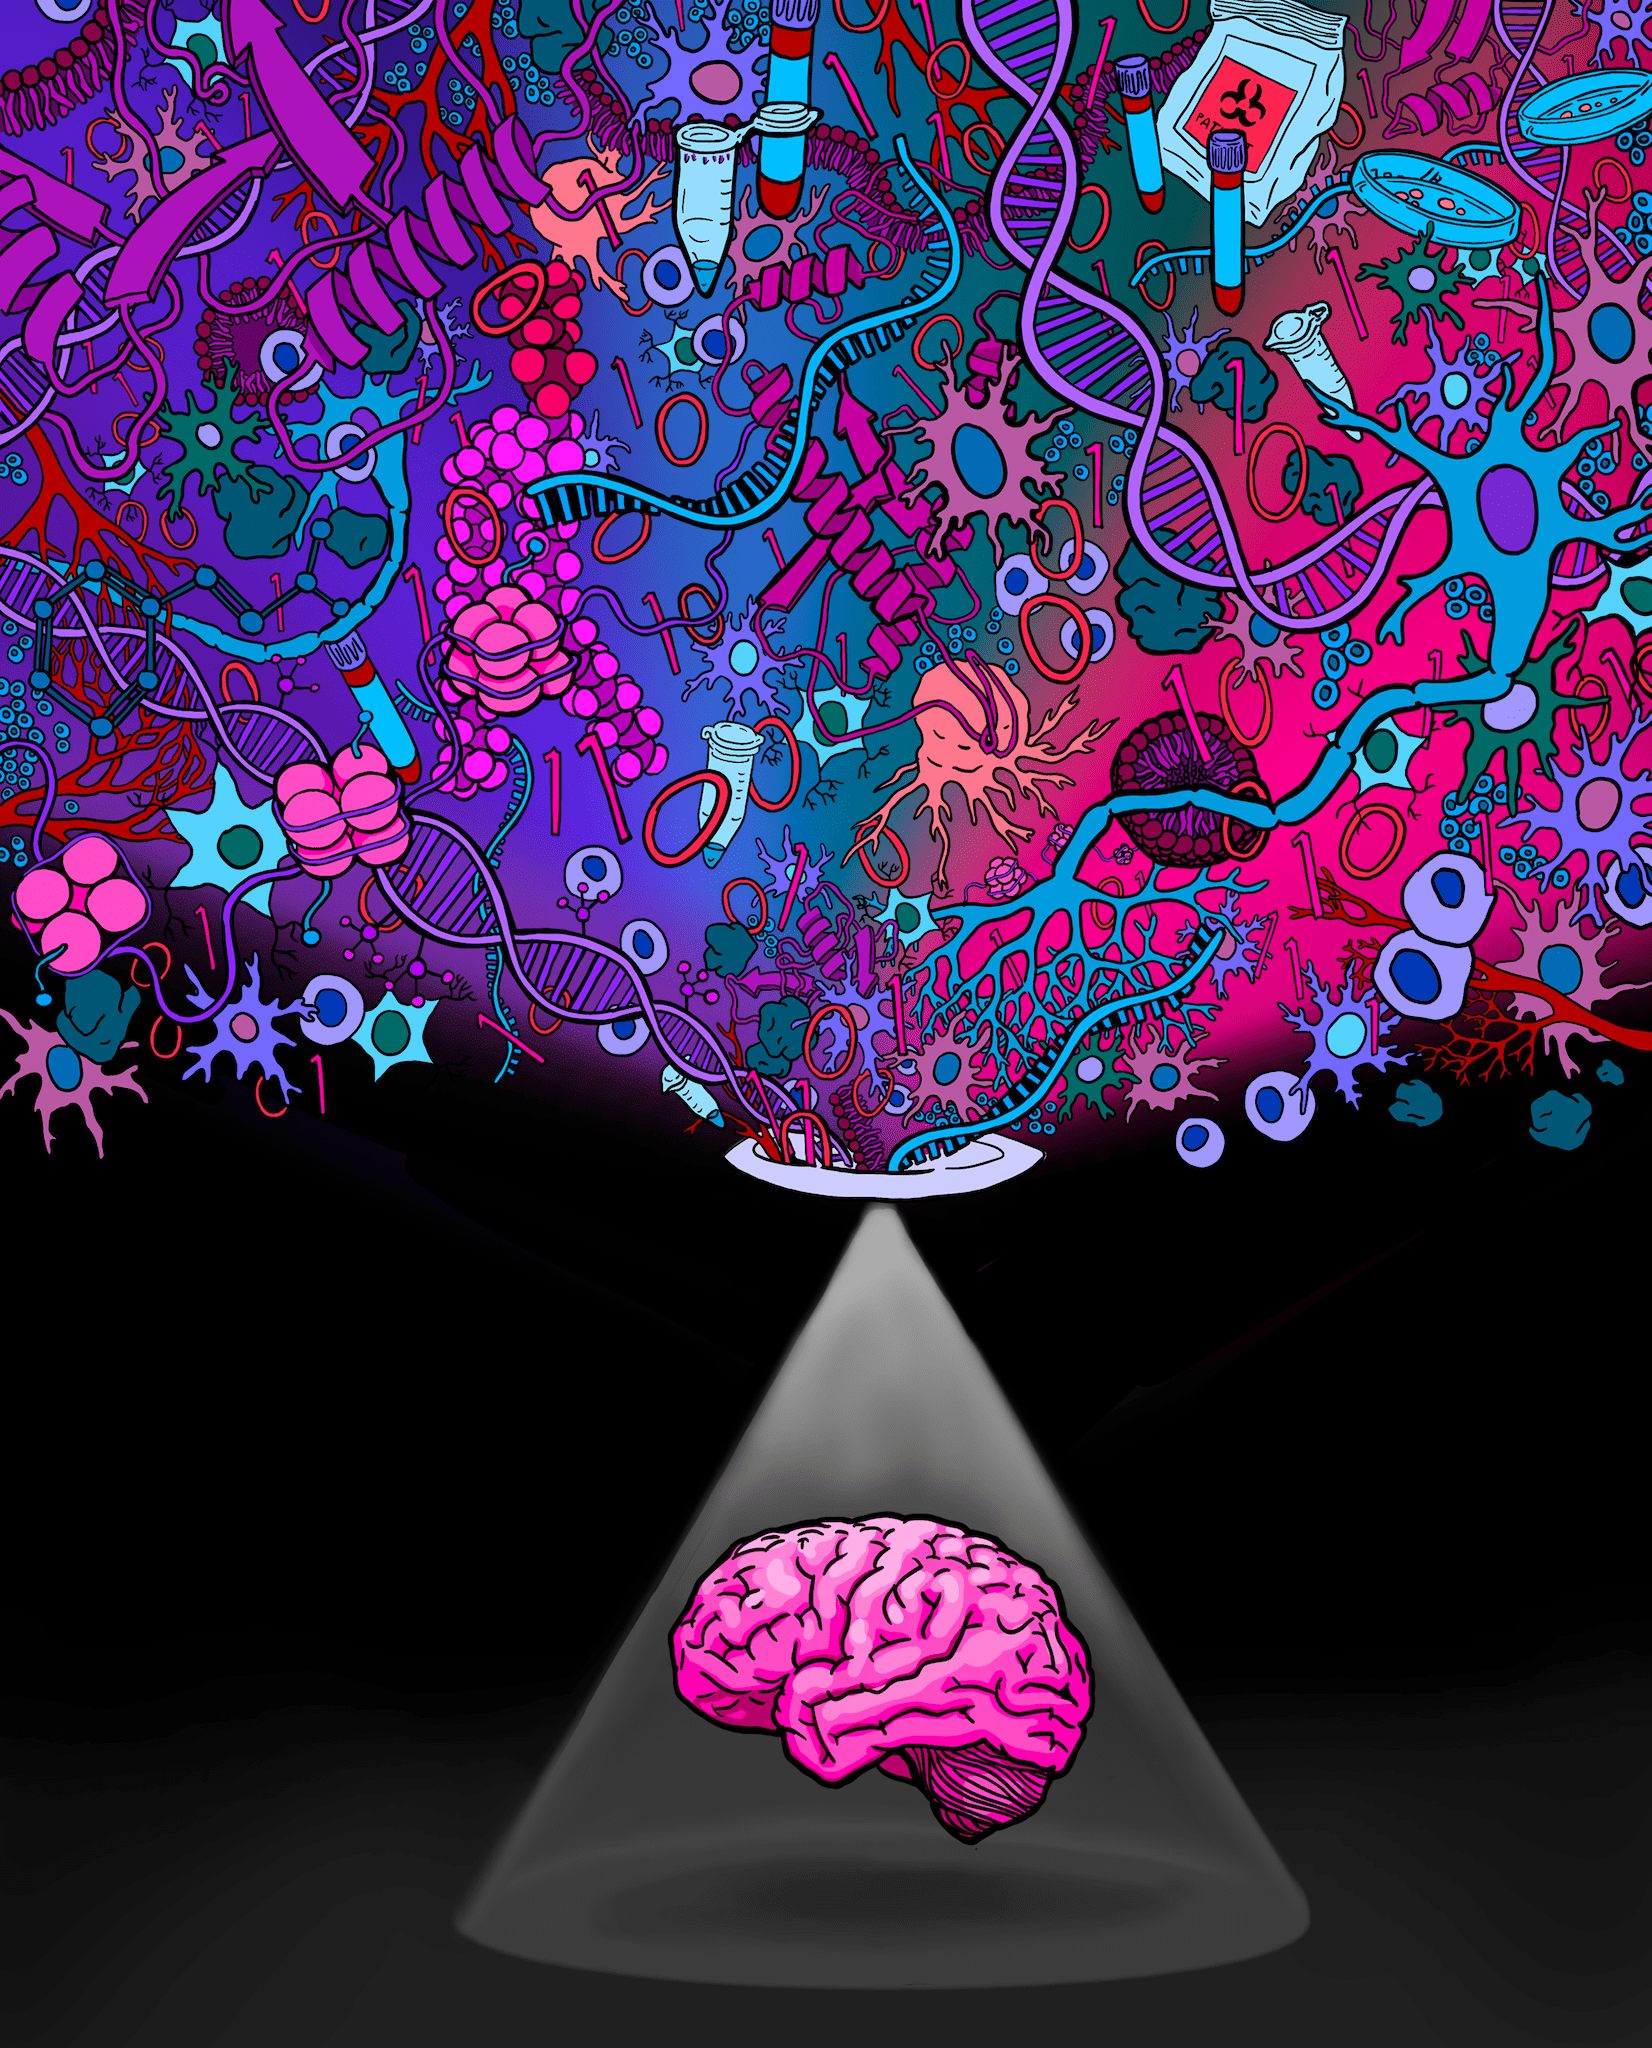
\includegraphics[width=0.6\linewidth]{figures/chap05_conclusion/cptac_gbm_cancer_cell_cover.png}
    \caption[Better disease understanding through a lens for an integrative view of multi-omics datasets.]{Better disease understanding through a lens for an integrative view of multi-omics datasets. Cover art of \textit{Cancer Cell} (April 2021 issue). Artwork by Jessica Johnson \url{https://jessicajohnsonart.com/}.}
    \label{fig:lens-multi-omics}
\end{figure}

\begin{figure}[tb]
    \centering
    \phantomlabel{fig:cptac-gbm-future-plan-longitudinal}
    \phantomlabel{fig:cptac-gbm-future-plan-heterogeneity}
    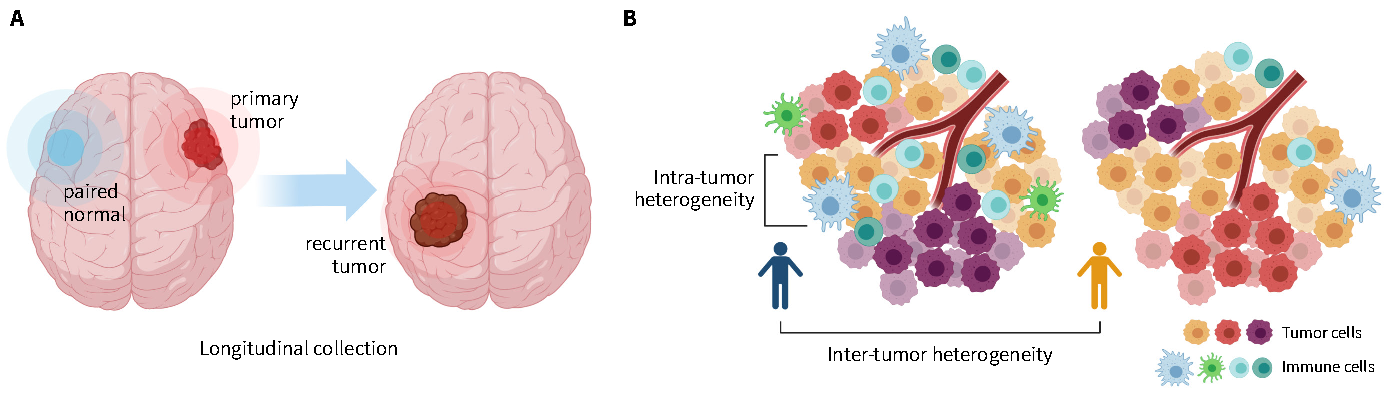
\includegraphics[width=1\linewidth]{figures/chap05_conclusion/gbm_future_plan.pdf}
    \caption[CPTAC GBM study future plan.]{%
        CPTAC GBM study future plan.
        \subref{fig:cptac-gbm-future-plan-longitudinal} Longitudinal collection of tumor samples and paired normal samples.
        \subref{fig:cptac-gbm-future-plan-heterogeneity} Tumor heterogeneity using single cell technologies.
    }
    \label{fig:cptac-gbm-future-plan}
\end{figure}
